%2multibyte Version: 5.50.0.2953 CodePage: 1252

\documentclass{article}
%%%%%%%%%%%%%%%%%%%%%%%%%%%%%%%%%%%%%%%%%%%%%%%%%%%%%%%%%%%%%%%%%%%%%%%%%%%%%%%%%%%%%%%%%%%%%%%%%%%%%%%%%%%%%%%%%%%%%%%%%%%%%%%%%%%%%%%%%%%%%%%%%%%%%%%%%%%%%%%%%%%%%%%%%%%%%%%%%%%%%%%%%%%%%%%%%%%%%%%%%%%%%%%%%%%%%%%%%%%%%%%%%%%%%%%%%%%%%%%%%%%%%%%%%%%%
\usepackage{amsfonts}
\usepackage{amsmath}

\setcounter{MaxMatrixCols}{10}
%TCIDATA{OutputFilter=LATEX.DLL}
%TCIDATA{Version=5.50.0.2953}
%TCIDATA{Codepage=1252}
%TCIDATA{<META NAME="SaveForMode" CONTENT="1">}
%TCIDATA{BibliographyScheme=Manual}
%TCIDATA{Created=Tuesday, September 13, 2016 11:26:35}
%TCIDATA{LastRevised=Tuesday, October 15, 2019 14:55:43}
%TCIDATA{<META NAME="GraphicsSave" CONTENT="32">}
%TCIDATA{<META NAME="DocumentShell" CONTENT="Standard LaTeX\Blank - Standard LaTeX Article">}
%TCIDATA{CSTFile=40 LaTeX article.cst}
\usepackage{enumitem}
\usepackage{floatrow}
\usepackage{graphicx} 
\usepackage{caption}

\newtheorem{theorem}{Theorem}
\newtheorem{acknowledgement}[theorem]{Acknowledgement}
\newtheorem{algorithm}[theorem]{Algorithm}
\newtheorem{axiom}[theorem]{Axiom}
\newtheorem{case}[theorem]{Case}
\newtheorem{claim}[theorem]{Claim}
\newtheorem{conclusion}[theorem]{Conclusion}
\newtheorem{condition}[theorem]{Condition}
\newtheorem{conjecture}[theorem]{Conjecture}
\newtheorem{corollary}[theorem]{Corollary}
\newtheorem{criterion}[theorem]{Criterion}
\newtheorem{definition}[theorem]{Definition}
\newtheorem{example}[theorem]{Example}
\newtheorem{exercise}[theorem]{Exercise}
\newtheorem{lemma}[theorem]{Lemma}
\newtheorem{notation}[theorem]{Notation}
\newtheorem{problem}[theorem]{Problem}
\newtheorem{proposition}[theorem]{Proposition}
\newtheorem{remark}[theorem]{Remark}
\newtheorem{solution}[theorem]{Solution}
\newtheorem{summary}[theorem]{Summary}
\newenvironment{proof}[1][Proof]{\noindent\textbf{#1.} }{\ \rule{0.5em}{0.5em}}
%\input{tcilatex}
\begin{document}


\begin{center} 
{\Large Problem Set 3}
\end{center}


\begin{exercise} %6.1-6.4 SW
This exercise refers to Table 1. The estimated regressions were computed using data for 2015 from the Current Population Survey. The data set consists of information on 7178 full-time, full-year workers. The highest educational achievement for each worker was either a high school diploma or a bachelor’s degree. The workers’ ages ranged from 25 to 34 years. The data set also contains information on the region of the country where the person lived, marital status, and the number of children. For the purposes of this exercise, let
\begin{itemize}
    \item[--] AHE = average hourly earnings
    \item[--] College = binary variable (1 if college, 0 if high school)
    \item[--] Female = binary variable (1 if female, 0 if male)
    \item[--] Age = age (in years)
    \item[--] Northeast = binary variable (1 if Region = Northeast, 0 otherwise)
    \item[--] Midwest = binary variable (1 if Region = Midwest, 0 otherwise)
    \item[--] South = binary variable (1 if Region = South, 0 otherwise)
    \item[--] West = binary variable (1 if Region = West, 0 otherwise) 
\end{itemize}

\begin{figure}[p!]
    \caption*{\sc \textbf{Table 1}}\label{tab1}
    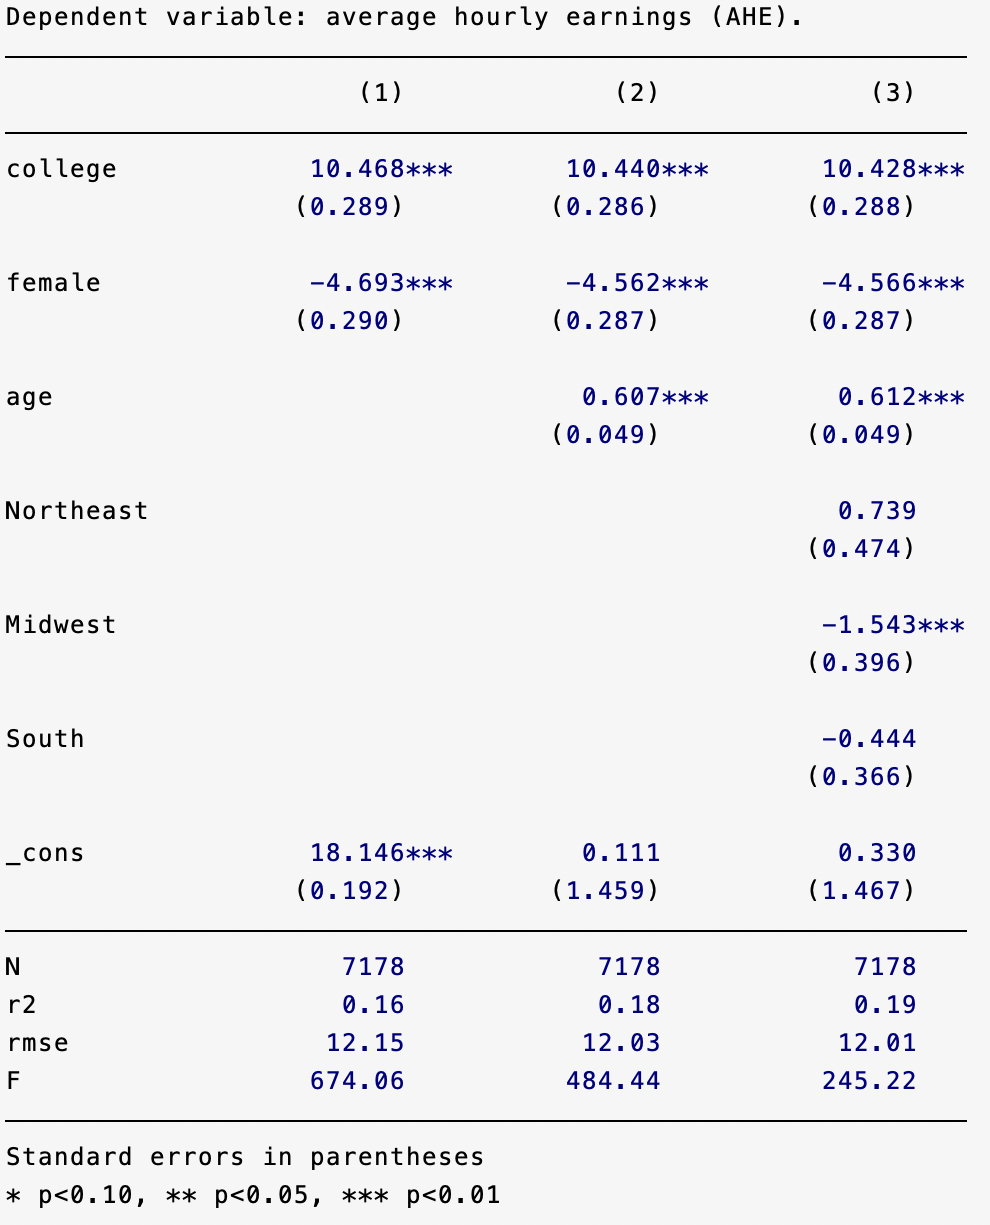
\includegraphics[width=1.2\textwidth]{images/PS3_ex1.png}
\end{figure}

    \begin{enumerate}[label=(\alph*)]
    \item Compute $\overline{R}^2$ for each of the regressions.
    \item Using the regression results in column (1):
    \begin{enumerate}[label=(\roman*)]
        \item Do workers with college degrees earn more, on average, than workers with only high school diplomas? How much more?
        \item Do men earn more than women, on average? How much more?
    \end{enumerate}
    \item Using the regression results in column (2):
    \begin{enumerate}[label=(\roman*)]
        \item Is age an important determinant of earnings? Explain.
        \item Sally is a 29-year-old female college graduate. Betsy is a 34-year-old female college graduate. Predict Sally’s and Betsy’s earnings.
    \end{enumerate}
    \item Using the regression results in column (3):
    \begin{enumerate}[label=(\roman*)]
        \item Do there appear to be important regional differences?
        \item Why is the regressor West omitted from the regression? What would happen if it were included?
        \item Celeste is a 28-year-old female college graduate from the South. Jennifer is a 28-year-old female college graduate from the Midwest. Calculate the expected difference in earnings between Celeste and Jennifer.
    \end{enumerate}
    \end{enumerate}
\end{exercise}



\begin{exercise}  %6.6 SW
A researcher plans to study the causal effect of a strong legal system on the
number of scandals in a country, using data from a random sample of countries
in Asia. The researcher plans to regress the number of scandals on how
strong a legal system is in the countries (an indicator variable taking the value
1 or 0, based on expert opinion).
    \begin{enumerate}[label=(\alph*)]
        \item Do you think this regression suffers from omitted variable bias? Explain why. Which variables would you add to the regression?
        \item Using the expression for omitted variable bias given in Equation (6.1), assess whether the regression will likely over- or underestimate the effect of a strong legal system on the number of scandals in a country. That is, do you think that $\hat{\beta_1}>\beta_1$ or $\hat{\beta_1}<\beta_1$?
    \end{enumerate}
\end{exercise}


\begin{exercise} %6.7 SW
Critique each of the following proposed research plans. Your critique should explain any problems with the proposed research and describe how the research plan might be improved. Include a discussion of any additional data that need to be collected and the appropriate statistical techniques for analyzing those data.
    \begin{enumerate}[label=(\alph*)]
        \item A researcher wants to determine whether a leading global university is guilty of racial bias in admissions. To determine potential bias, the researcher collects data on the race of all applicants to the university for a given year. The researcher plans to conduct a difference-in-means test to determine whether the proportion of acceptances among Black candidates is systematically different from the proportion of acceptances among other candidates.
        \item A researcher is interested in identifying the impact of a mother’s education on the educational attainment of her child. She collects data on a random sample of individuals aged between 25 and 40 years who are out of the schooling system. The data set contains information on each person’s level of schooling, the type of school attended, gender and ethnicity, as well as information on the schooling of their parents and the demographic characteristics of the household in which they grew up. The researcher plans to regress years of schooling achieved by an individual on the years of schooling of their mother, including in the regression the other potential determinants of schooling (number of siblings and whether parents lived together or are separated) as controls.
    \end{enumerate}

\end{exercise}


\begin{exercise} %6.11 SW
Consider the regression model
\begin{equation*}
    Y_i = \beta_1 X_{1i} + \beta_2 X_{2i} + u_i
\end{equation*}
for $i = 1, \dots, n$. Notice that there is no constant term in the regression.
    \begin{enumerate}[label=(\alph*)]
    \item Specify the least squares function that is minimized by OLS.
    \item Compute the partial derivatives of the objective function with respect to
$\beta_1$ and $\beta_2$.
    \item Suppose that $\sum_{i=1}^n  X_{1i}X_{2i}=0$. Show that $\hat{\beta}_1=\sum_{i=1}^n X_{1i}Y_i/\sum_{i=1}^n X_{1i}^2$
    \item Suppose that $\sum_{i=1}^n  X_{1i}X_{2i}\neq0$.Derive an expression for $\hat{\beta}_1$ as a function of the data $(Y_i,  X_{1i}, X_{2i}), i = 1, \dots, n$
    \item Suppose that the model includes an intercept: $ Y_i = \beta_0 + \beta_1 X_{1i} + \beta_2 X_{2i} + u_i$. Show that the least squares estimators satisfy $\hat{\beta}_0=\overline{Y}-\hat{\beta}_1\overline{X}_{1}-\hat{\beta}_2\overline{X}_{2}$
    \item As in (e), suppose that the model contains an intercept. Also, suppose that $\sum_{i=1}^n  (X_{1i}-\overline{X}_{1})(X_{2i}-\overline{X}_{2})=0$. Now show that $\hat{\beta}_1=\sum_{i=1}^n (X_{1i}-\overline{X}_{1})(Y_{i}-\overline{Y})/\sum_{i=1}^n (X_{1i}-\overline{X}_{1})^2$. How does this compare to the OLS estimator of $\beta_1$ from the regression that omits $X_2$?
    \end{enumerate}
\end{exercise}


\begin{exercise}  %7.7 SW
Data were collected from a random sample of 200 home sales from a community in 2013. Let Price denote the selling price (in \$1000s), BDR denotes the number of bedrooms, Bath denotes the number of bathrooms, Hsize denotes the size of the house (in square feet), Lsize denotes the lot size (in square feet), Age denotes the age of the house (in years), and Poor denote a binary variable that is equal to 1 if the condition of the house is reported as “poor.” An estimated regression yields
\begin{equation*}
    \begin{alignedat}{5}
    \widehat{Price}
    = 109&.7 &{}
    +0&.567 \times \mathrm{BDR} &{}
    + 26&.9 \times \mathrm{Bath} &{}
    + 0&.239 \times \mathrm{Hsize} &{}\\
    (22&.1)& (1&.23)& (9&.76)& (0&.021)\\\\
 + 0&.005 \times \mathrm{Lsize} &{}
    + 0&.1 \times \mathrm{Age} &{}
    - 56&.9 \times \mathrm{Poor} &{} \\
(0&.00072)& (0&.23)& (12&.23)&
  \end{alignedat}
\end{equation*}
with $\overline{R}^2=.85$ and $SER = 45.8$.

    \begin{enumerate}[label=(\alph*)]
    \item Is the coefficient on BDR statistically significantly different from zero?
    \item Typically, four-bedroom houses sell for more than three-bedroom houses. Is this consistent with your answer to (a) and with the regression more generally?
    \item A homeowner purchases 2500 square feet from an adjacent lot. Construct a 95\% confidence interval for the change in the value of her house.
    \item Lot size is measured in square feet. Do you think that another scale might be more appropriate? Why or why not?
    \item The F-statistic for omitting BDR and Age from the regression is F = 2.38. Are the coefficients on BDR and Age statistically different from zero at the 10\% level?
    \end{enumerate}
    
\end{exercise}



\end{document}
